%!TEX root = proyecto.tex

\chapter{Diseño y resolución}

%\linespread{1.5}

\section{Paul Viola and Michael Jones} \label{haar-like}

En 2001, el reconocimiento facial tuvo su primera aparición en el campo de la visión artificial como aplicación en tiempo real. Este avance fue de la mano de Paul Viola y Michael Jones. Análogamente, el punto de partida del estudio de este TFG. Durante este apartado, se estudiará el funcionamiento del algoritmo \textit{Viola-Jones face detector}, ideado por estos dos investigadores y se realizará una implementación del mismo mediante \textit{Python} y \textit{OpenCV} para comprobar como se comporta en la situación actual.

\subsection*{Método de estudio}

El trabajo de los expertos fue presentado por parte de la Universidad de Cambridge mediante un \textit{paper} (ensayo de la investigación). Y se introduce como: 
\begin{quote}
	"[...] This paper describes a machine learning approach for visual object detection which is capable of processing images extremely rapidly and achieving high detection rates" \cite{paulViola}
\end{quote}

Para poder lograr esta afirmación se basan en un procedimiento de trabajo en dos fases: entrenamiento y detección. Igualmente, Paul y Michael dividen el proyecto en tres ideas principales para poder lograr un detector que se pueda ejecutar en tiempo real. Y estas son: la imagen integral, Adaboost (algoritmo de Machine Learning) y un método llamado \textit{attentional cascade structure}. 

Con todos estos puntos combinados lograron ingeniar un prototipo capaz de detectar caras humanas con un \textit{frame rate} de 15 fps. Fue diseñado para la detección de caras frontales, haciéndose difícil para posiciones laterales o inclinadas.

Las imágenes que se toman para realizar la detección pasan por una transformación del espacio de color a \textit{grayscale}. Con el objeto de encontrar características en ellas, llamadas \textit{haar-like features}. Nombradas así por su inventor Alfred Haar en el siglo XIX. En este trabajo se hacen uso de tres tipos de haar-like features (Figura \ref{fig:haarLike}).

\begin{figure}[htp]
	\centering
	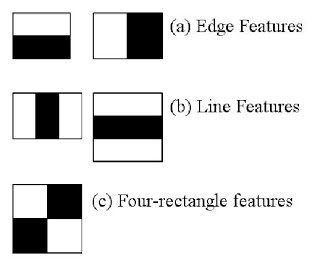
\includegraphics[width=5cm]{imagenes/haar-like.jpeg}
	\caption{Haar-like Features \cite{haar-like}.}
	\label{fig:haarLike}
\end{figure}

Las \textbf{\textit{Haar-like features}}, o también conocidas como \textit{Haar-wavelet} son una secuencia de funciones \textit{rescaled square-shaped}, siendo similares a las funciones de Fourier y con un comportamiento parecido a los \textit{Kernel} usados en las \textit{Redes Convolucionales} (matrices que consiguen extraer ciertas \textit{features} de la imagen de entrada). De manera que, las \textit{Haar Features} serán las características de la detección facial.

En un estudio ideal, los píxeles que forma el \textit{feature} tendrá una división clara entre píxeles de color blanco con los de color negro (Figura \ref{fig:haarLike}), pero en la realidad eso casi nunca se va a dar.

Más específicamente, las \textit{Haar-like features} están compuestas por valores escalares que representan la media de intensidades entre dos regiones rectangulares de la imagen. Estas capturan la intensidad del gradiente, la frecuencia espacial y las direcciones, mediante el cambio del tamaño, posición y forma de las regiones rectangulares basándose en la resolución que se define en el detector \cite{haar-like}. 

Estas características van a ayudar al ordenador a entender lo que es la imagen estudiada. Van a ser utilizadas mediante \textit{Machine Learning} para detectar donde hay una cara o no, mediante un recorrido sobre toda la imagen. Esto conlleva una potencia de computación elevada. Para paliar este problema idearon el método de la \textit{Imagen Integral}.

La \textbf{\textit{Imagen Integral}} permite calcular sumatorios sobre subregiones de la imagen, de una forma casi instantánea. Además de ser muy útiles para las \textit{HAAR-like features}, también lo son en muchas otras aplicaciones.

Si se supone una imagen con unas dimensiones de $<w,h>$ (ancho y alto, respectivamente), la imagen integral que la representa tendrá unas dimensiones de $<w+1,h+1>$. La primera fila y columna de esta son ceros, mientras que el resto tendrán el valor de la suma de todos los píxeles que le preceden \cite{integral-web}. Ahora, para calcular la suma de los píxeles en una región especifica de la imagen, se toma la correspondiente en la imagen integral y se suma según la siguiente fórmula (siguiendo la numeración de la Figura \ref{fig:integral}):
\begin{center}
	$sum = L4 + L1 - (L2 + L3)$ 
\end{center}
\begin{figure}[htp]
	\centering
	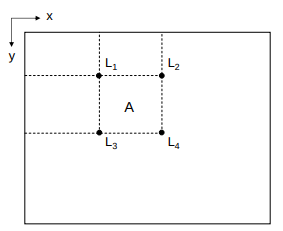
\includegraphics[width=5cm]{imagenes/integral.png}
	\caption{Funcionamiento de una \textit{Imagen Integral} \cite{integral-web}.}
	\label{fig:integral}
\end{figure}

Viola y Jones junta esta propuesta con los filtros \textit{Haar-like features}, y consiguen computar dichas características de manera constante y eficaz \cite{integral}.

% ---------------------------
%https://aishack.in/tutorials/integral-images-opencv/

%https://www.quora.com/How-integral-image-is-used-in-image-processing-and-how-improves-the-computation-time?share=1
%https://www.quora.com/What-are-the-must-read-papers-in-the-field-of-computer-vision-for-a-student-in-pursuing-research-in-the-field
% ---------------------------
%
% MACHINE LEARNING - ADABOOST
Una vez estudiada la obtención de características y con un set de entrenamiento, solo queda seleccionar un método de \textit{Machine Learning} que permita crear una función de clasificación. Concretamente, se plantea el uso de una variante de \textbf{\textit{AdaBoost}}, que permite seleccionar un pequeño conjunto de características y poder entrenar un clasificador. 

Este algoritmo de aprendizaje esta basado en generar una predicción muy buena a partir de la combinación de predicciones peores y más débiles, donde cada uno de estas se corresponde con el \textit{threshold} de una de las características \textit{Haar-like}. La primera vez que aparece este algoritmo, de forma práctica, fue de la mano de \textit{Freund y Schapire} \cite{adaboost1}. Sin embargo, el usado por \textit{Viola y Jones} es una modificación de este. La salida que genera el algoritmo \textbf{\textit{AdaBoost}} es un clasificador llamado \textit{Strong Classifier}, como se ha mencionado anteriormente, compuesto por combinaciones lineales de \textit{Weak Classifiers}. 

El procedimiento para encontrar \textit{Weak Classifiers} es ejecutar el algoritmo T iteraciones donde T es el número de clasificadores a encontrar. En cada iteración, el algoritmo busca el porcentaje de error entre todas las características y escoge la que menos porcentaje de error presente en dicha iteración \cite{adaboost2}. (Como se muestra en la \textit{Figura \ref{fig:ada1}}) 

\begin{figure}[htp]
	\centering
	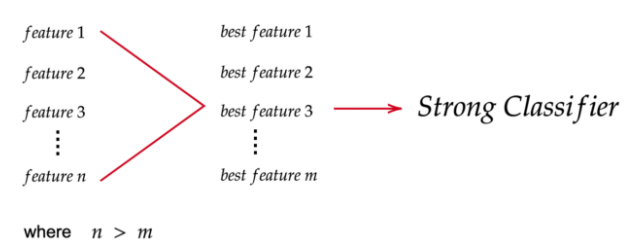
\includegraphics[width=10cm]{imagenes/ada1.png}
	\caption{Construcción del \textit{Strong Classifier} \cite{adaboost2}.}
	\label{fig:ada1}
\end{figure}

Con estos clasificadores se procede a la construcción de una estructura en cascada para crear un \textit{Multi-stage Classifier}, que podrá realizar una detección rápida y buena. Por tanto, la estructura de cascada esta compuesta por varios estados de \textit{Strong Classifiers} generados por el algoritmo \textit{AdaBoost}. Donde el trabajo de cada estado será identificar si, dada una región de la imagen, no hay una cara o si hay la posibilidad de que la haya \cite{adaboost1}. Si el resultado de uno de los estados es que no existe una cara en dicha región, esta se descarta directamente. Mientras que, si hay la posibilidad de que exista una, pasa al siguiente estado de la estructura. De tal forma que, cuantos más estados atraviese una región de la imagen, con más seguridad se podrá afirmar que existe una cara en ella. La estructura completa se refleja en la \textit{Figura \ref{fig:ada2}}.

\begin{figure}[htp]
	\centering
	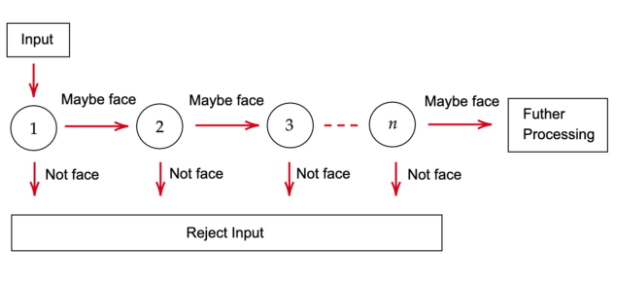
\includegraphics[width=8cm]{imagenes/ada2.png}
	\caption{Construcción del \textit{Multi-stage Classifier} \cite{adaboost2}.}
	\label{fig:ada2}
\end{figure}

% VIDEO DE LOCOS: https://www.youtube.com/watch?v=uEJ71VlUmMQ&t=5s

\subsection*{Implementación y Experimentación}

El prototipo será implementado en \textit{Python}, con el uso de \textit{OpenCV}. Y, el objetivo es construir dos detectores de caras, donde el primero usará dos modelos preentrenados de \textit{OpenCV} de caras frontales, para estudiar cual es mejor para el siguiente prototipo. Mientras que en el segundo, se intentará modificar el programa, para que mediante el uso de uno de estos modelos preentrenados y uno de \textit{Machine learning} se pueda detectar una cara con una mascarilla o sin ella.

La \textbf{implementación básica} hace uso de un modelo preentrenado cargado mediante una clase de \textit{OpenCV}, llamada \textit{Cascade Classifier}. Esta representa la base de \textit{Machine Learning} explicado en el apartado anterior. Asimismo, \textit{OpenCV} también proporciona una serie de archivos \textit{xml} con diferente modelos preentrenados. En concreto, para este prototipo se hace uso del modelo por defecto, detector de caras frontal, como se muestra en la investigación de \textit{Viola y Jones}, y una variante del mismo denominada \textit{frontalface\_alt2.xml}. Finalmente, la detección se realiza, tras hacer una transformación del espacio de color a blanco y negro, mediante la función \textit{detectMultiScale} de la clase, creada anteriormente, \textit{Cascade Classifier}. Concretamente, su funcionalidad será encontrar caras dentro de las imágenes que vaya procesando.

La prueba de esta prototipo se realizará a una distancia corta (70 cm)  y media (150 cm), para comprobar su funcionamiento estandar con dos modelos pre-entrenados, llamados:  \textit{frontalface\_default.xml} y \textit{frontalface\_alt2.xml}, dedicados a reconocer rostros de manera frontal. Intentando estudiar su velocidad de procesamiento y su precisión a la hora de detectar un rostro sin y con obstáculos, el resultado obtenido se ve reflejado en la \textit{Figura \ref{fig:haar1}}.

\begin{figure}[htp]
	\centering
	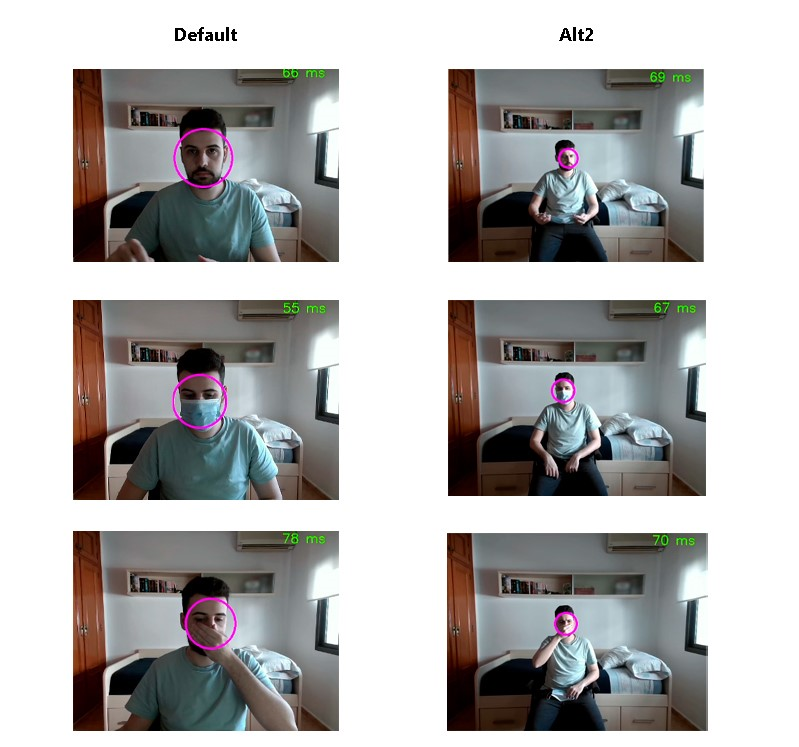
\includegraphics[width=10cm]{imagenes/prueba_proto1.jpg}
	\caption{Pruebas con Haar-like features con: \textit{frontalface\_default.xml} y \textit{frontalface\_alt2.xml}}
	\label{fig:haar1}
\end{figure}

Tras la experimentación se puede comprobar que ambos modelos funcionan bastante bien, tanto para un reconocimiento de rostro sin obstáculos como con ellos. Aunque, es importante destacar que el modelo pre-entrenado \textit{frontalface\_default.xml} no es tan preciso en distancias superiores a los 150 cm. En cuanto a los tiempos recogidos para estas pruebas, el segundo modelo pre-entrenado \textit{frontalface\_alt2.xml} obtiene un tiempo medio más lento pero funciona de forma más precias. Se refleja en la siguiente tabla:

\begin{table}[h!]
	\begin{center}
		\begin{tabular}{ |c|c|c|c|c|c| } 
			\hline
			& default (70cm) & default (150cm) & alt2 (70cm) & alt2 (150cm) \\
			\hline
			PC1 / Time (MS) & 46.15  & 45.09 & 62.04  & 61.75 \\
			\hline
			PC2 / Time (MS) & X  & X & X  & X \\
			\hline
		\end{tabular}
		\caption{Tiempos para el prototipo 1.}
		\label{tab:table2}
	\end{center}
\end{table}

El \textbf{segundo prototipo} (custom) implementa un identificador de caras conjunto a un modelo de \textit{Machine Learning} que identifica cuando una persona lleva o no mascarilla, además de si se lleva bien. Gracias a los modelos PCA y SVM, se puede crear un modelo para su identificación con el uso de muestras de los modelos pre-entrenados \textit{Haar-like features} probados antes. Para ello se realizará el siguiente esquema de procedimiento:

\begin{enumerate}
	\item Haar-like features
	
	Sigue el mismo procedimiento que el prototipo anterior. Mediante la creación de una clase de OpenCV, llamada \textit{CascadeClassifier}, y el uso de un modelo \textit{Haar-like features} pre-entrenado, se obtiene el ROI donde se localiza un rostro. En este caso, se hará un estudio con el modelo pre-entrenado llamado \textit{frontalface\_alt2.xml}, capaz de reconocer de forma más fiable rostros con mascarilla. 
	
	\item Modelo PCA/SVM
	
	Una vez obtenido el ROI de la localización de la cara con o sin mascarilla, se procede a predecir de que caso se trata. Previo a dicha predicción y ejecución del prototipo, se necesita entrenar el modelo. Y para ello se toman referencias de rostros con y sin la mascarilla para que sirvan como entrada en el entrenamiento del modelo, usando el prototipo anterior. Exactamente se debe ejecutar dos veces el archivo \textit{Python: trainCascade.py}, una para el caso de sin y otro para el caso de con mascarilla. Siendo la mejor opción, el uso del modelo pre-entrenado \textit{frontalface\_alt2.xml}. También es posible realizar el entrenamiento con imágenes de un dataset.
	
	Principal Component Analysis, (\textbf{PCA}), es un algoritmo de \textit{Machine Learning} dedicado a la reducibilidad de dimensionalidad. Identifica un hiperplano común que conecta a todos los datos y son proyectados sobre él. \textit{Scikit-Learn} ofrece una implementación de este, mediante descomposición SVD (Singular Value Decomposition), también conocido como una regresión lineal \cite{geron_2020}. La salida de PCA servirá para reducir la complejidad de la entrada al modelo \textbf{SVM} (Support Vector Machine), capaz de realizar regresiones o clasificaciones tanto lineales como no lineales. La idea tras este modelo es separar los distintos conjuntos de datos existentes mediante lineas rectas en el espacio (Figura \ref{fig:svm}) \cite{geron_2020}.
	
	\begin{figure}[htp]
		\centering
		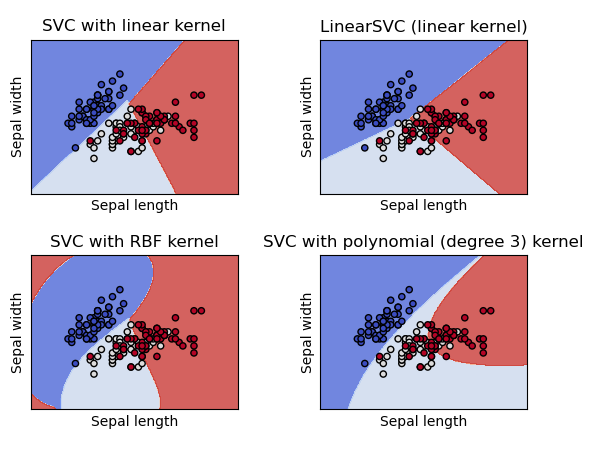
\includegraphics[width=7cm]{imagenes/svm_example.png}
		\caption{Ejemplos de clasificaciones SVM}
		\label{fig:svm}
	\end{figure}

	Para la implementación de esta parte se hace uso de \textit{Scikit-Learn}, librería de Python que implementa una gran variedad de clasificadores, regresores y cluster de modelos \textit{Machine Learning}.
\end{enumerate}

En resumen, el procedeminiento que sigue este prototipo se basa en cargar el modelo que se ha creado, detectar un rostro en al imagen de entrada y a partir de ese ROI (donde se encuentra dicho rostro), hacer un estudio con el modelo y mostrar por pantalla el resultado. Para la detección de los rostros antes de tratarlos con el modelo se realizará con el modelo pre-entrenado \textit{frontalface\_default.xml}, para conseguir un funcionamiento más fluido. El funcionamiento del prototipo se muestra en la Figura \ref{fig:haarCustom}.

\begin{figure}[htp]
	\centering
	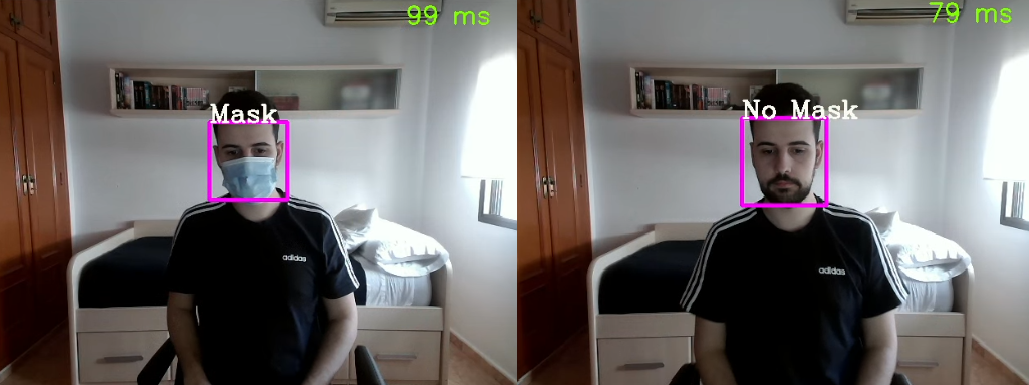
\includegraphics[width=15cm]{imagenes/haarcustom_prueba.png}
	\caption{Pruebas con prototipo Haar Custom}
	\label{fig:haarCustom}
\end{figure}

La desventaja es que solamente funciona con los rostros/rostro que se toma como referencia para construir el modelo, igualmente pasa con el tipo de mascarilla (siendo la quirúrgica la que mejor funciona con este prototipo). Asimismo, su funcionamiento es de manera frontal y cercana, tanto a 70 cm como a 150 cm, funciona de forma correcta. Sin embargo, para una posición lejana y con más información a tratar el detector se pierde y crea identificaciones falsa o no llega a reconocer nada. Asimismo, el tiempo de retardo que presenta este prototipo para el PC1 es de una media de 87.5 ms.

Este procedimiento se podría llegar a usar con otra implementación, específicamente con HOG, centrada también en la extracción de caracteristicas pero usando gradientes.

\newpage
\section{Facial Landmark}

Con el objetivo de ampliar la idea anterior, se plantea el uso de Facial Landmark, una tecnología que nos permite el reconocimiento de puntos de interés en las caras que se han detectado en la imagen. Sus pasos de ejecución son: detectar cara dentro de la imagen (En este caso, se usará \textit{Haar-like features}) y obtener dichos puntos de interés. La implementación que se va a utilizar es la estudiada por \textit{Kazemi} y \textit{Sullivan} en 2014, con el paper \textit{One Millisecond Face Alignment with an Ensemble of Regression Trees} \cite{inproceedings}, y usado en el \textit{toolkit} \textit{Dlib}. Este método se centra en localizar las siguientes zonas faciales: boca, cejas, ojos, nariz y mentón, gracias al uso de un conjunto de árboles de regresión. Estos son entrenados mediante  un modelo formado por puntos de interés de un grupo de imágenes, etiquetados a mano y especificadas como coordenadas (x,y). 

\textit{Dlib} será el \textit{toolkit} (\textit{Open Source}) utilizado para la implementación de dicho método. Este contiene algoritmos de \textit{Machine Learning} y herramientas capaces de crear software complejo en \textit{C++} y \textit{Python} para resolver problemas reales. Sobre todo centrado en robótica, dispositivos embebidos, móviles y ordenadores de gran capacidad \cite{dlib}. 

\subsection*{HOG - \textit{Histogram of Oriented Gradients}}

El primer paso en esta solución es encontrar una cara dentro de la imagen de entrada, y el encargado será el método HOG. El cual, sigue una idea similar al método de \textit{Haar-like}, ya que se basa en la detección de \textit{features} (características).

La idea teórica tras \textit{HOG} es encontrar la apariencia y forma de un objeto mediante la distribución de la intensidad de gradientes locales, gracias a que estos obtienen una magnitud mayor en las cercanías de bordes o esquinas. Mientras que la implementación, divide la imagen en pequeñas regiones (llamadas celdas) y se calcula un histograma de gradientes de una dimensión para cada uno de los píxeles de cada celda. Para un mejor estudio se normaliza el contraste de la imagen de entrada \cite{hog}. Con este procedimiento se obtiene un \textit{feature vector} a partir de la imagen de entrada, y la distribución resultante de los gradientes serán usados como las características. La implementación de HOG se podría dividir en 5 pasos generales \cite{hog2}:

\begin{enumerate}
	\item \textit{Pre-procesado}: Para una imagen de entrada de cualquier tamaño es tratada en regiones de ciertas escalas y analizadas en varias zonas de la imagen. La única restricción es que los tamaño de las regiones analizadas tienen una relación de aspecto fija.
	
	\item \textit{Cálculo de las imágenes de gradiente}: Para el calculo del histograma de gradientes es necesario realizar el cálculo de los gradientes, tanto verticales como horizontales. Esto se puede obtener fácilmente gracias al uso de \textit{Kernels} (filtros). Posteriormente, se busca la magnitud de las direcciones de dichos gradientes con el uso de la siguiente fórmula:
	
	\begin{figure}[htp]
		\centering
		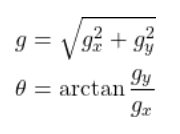
\includegraphics[width=3cm]{imagenes/HOGFormula.png}
		\caption{Fórmula \textit{HOG} \cite{hog2}.}
		\label{fig:hogf}
	\end{figure}
	
	La fórmula esta implementada en \textit{OpenCV} mediante la función \textit{cartToPolar}. En este punto se puede obtener la imagen de los gradientes, eliminando toda la información no relevante de la imagen original, observando como en todos los píxeles el gradiente tomarán una magnitud y una dirección. Si la imagen es RGB, los gradientes se evalúan sobre los tres canales de color, siendo la magnitud final el valor mayor entre los tres canales.
	
	\item \textit{Cálculo de los histogramas de gradientes en celdas (8x8)}: La imagen se divide en celdas y se calculan los histogramas para cada una de ellas. Por ejemplo, si la celda es de tamaño 8x8, esta contendrá 192 píxeles (8x8x3), donde el gradiente tiene dos valores, descritos anteriormente (magnitud y dirección), por cada uno de los píxeles, lo que añade 128 valores (8x8x2). Esto facilita la representación de las regiones mediante el uso de un histograma, además mejora la influencia al ruido. El tamaño de la celda vendrá definida dependiendo de la escala de características (\textit{features}) que se estén buscando.
	
	\item \textit{Normalización de bloques (16x16)}: Una vez creado el histograma, hay que tener en cuenta que la imagen es sensible al brillo que tenga. Por ejemplo, si el brillo de la imagen se divide en dos, la magnitud del gradiente también lo hará. De igual forma, si el brillo se multiplica por dos, el gradiente ídem. Pero, se busca un descriptor que sea independiente a esto, por lo que se normaliza el histograma para que no se vea afectado por los cambios de luz/brillo.	Disponiendo de celdas de 8x8, un bloque de 16x16 posee cuatro histogramas que pueden ser condensados en un único vector normalizado.
	
	\item \textit{Cálculo del vector de HOG}: El último paso es concatenar los vectores normalizados obtenidos en uno global.

\end{enumerate}

Este procedimiento se repite varias veces sobre imágenes distintas y se introduce en un modelo \textit{Machine Learning} del tipo SVM Linear, con el objetivo de obtener un detector de caras. En el caso de \textit{Dlib}, posee un modelo preentrenado.


\subsection*{Sullivan Paper}

El \textit{paper} de Kazemi y Sullivan presenta la implementación usada en el \textit{toolkit Dlib} del algoritmo que estima de forma precisa y eficiente los puntos de interés faciales. Esta basado en \textit{gradient boosting} para el aprendizaje de un conjunto de arboles de regresión (\textit{ensemble of regression trees}), que será el encargado de la predicción de los puntos de interés \cite{faceLandmark}.

Este método fue uno de los primeros que mejoró el rendimiento, a diferencia con los métodos anteriores, gracias a la detección de componentes esenciales para el \textit{face aligment} y procesarlos para introducirlos en funciones de regresión en cascada. Cada una de estas funciones estima, de forma eficiente, la forma facial desde una estimación inicial y obtiene un conjunto de píxeles indexados a dicha estimación. En concreto, \textit{Dlib} estimará un total de 68 píxeles indexados (Figura \ref{fig:dlibPoints}), ya que sigue las anotaciones del \textit{dataset iBUG 300-W} \cite{ibug}, usado en los modelos pre-entrenados ofrecidos por \textit{Dlib}.

\begin{figure}[htp]
	\centering
	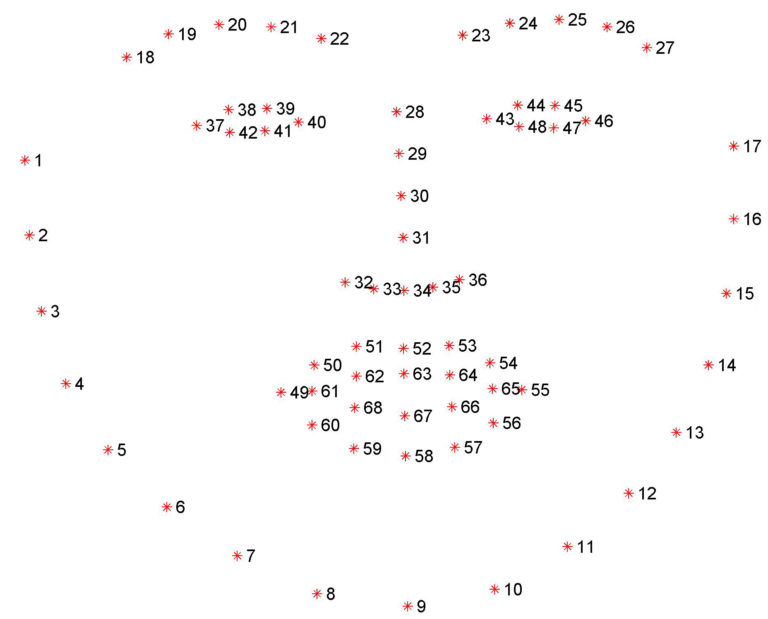
\includegraphics[width=8cm]{imagenes/facial_landmarks_68markup.jpg}
	\caption{68 coordenadas del \textit{facial landmark} con \textit{iBUG 300-W} \textit{dataset} \cite{ibug}.}
	\label{fig:dlibPoints}
\end{figure}

Además, se introdujeron dos elementos clave a las funciones de aprendizaje de regresión. El primero gira en torno a la intensidad de los píxeles indexados con respecto a la estimación actual de la forma facial, ya que estos son muy influenciables por la deformación de la estimación de la forma y a los cambios de iluminación. El dilema que aparece es que necesitamos características confiables para obtener una predicción con precisión la forma y, por otro lado, necesitamos una estimación precisa de la forma para extraer características fiables. Para resolver este dilema se plantea el uso de un enfoque iterativo. La idea se basa en obtener una imagen transformada en un sistema de coordenadas normalizado basado en una estimación actual de la forma, y posteriormente extraer las características para predecir un vector de actualización para los parámetros de la forma. Este proceso suele repetirse varias veces.

El segundo elemento clave se trata de reducir la dificultad del proceso de inferencia/predicción. El objetivo es obtener una función capaz de estimar la forma que concuerde con la información de la imagen y el modelo. 
%Pero el problema es que esta función es no convexa en varios valores locales.
Para resolver esto se plantearon dos soluciones a lo largo del tiempo. El primero afirma que las predicciones estimadas en zonas lineales del subespacio mienten, lo que concluyo siendo de ayuda para evitar este problema. Pero, posteriormente se descubrió una segunda solución, donde se asume que la función miente en zonas lineales del subespacio pero no es necesario realizar trabajo adicional. En el caso de este \textit{paper}, se implementa una solución donde se utilizan una combinación de ambas. Por lo que, cada regresor aprende mediante \textit{gradient boosting} conjuntamente a una función de perdida de error al cuadrado.
%La entrada usada en el regresor, es seleccionada mediante \textit{gradient boosting} sobre un conjunto de píxeles dispersos, y la prioridad de probabilidad sobre la distancia entre pares de píxeles de entrada. 
Esto permite realizar un estudio sobre un mayor número de características relevante de forma eficiente. El resultado es una cascada de regresores que pueden localizar los puntos de referencia faciales cuando es inicializada con la media de la pose facial \cite{faceLandmark}.

\newpage
De forma más general, la investigación ofrece las siguiente contribuciones a las investigaciones de \textit{Face Landmark} anteriores:

\begin{enumerate}
	\vspace{-0.2cm}
	\item Un método de alineación basado en un conjunto de árboles de regresión que devuelve la forma facial mientras minimiza la función de error.
	\vspace{-0.2cm}
	\item Método que maneja la predicción de puntos que faltan o no están presentes en la imagen. Por ejemplo, rostros que estén medio ocultos. (Esto solamente se realizará si el modelo creado con HOG detecta dicha cara oculta).
	\vspace{-0.2cm}
	\item Resultados donde se demuestran que el método produce predicciones de alta calidad.
	\vspace{-0.2cm}
	\item El efecto de la cantidad de datos de entrenamiento.
\end{enumerate}

\vspace{-0.8cm}
\subsection*{Prototipo}
\vspace{-0.5cm}
Mediante \textit{OpenCV} y el \textit{ToolKit Dlib} se obtiene la implementación de ambas ideas, mediante modelos pre-entrenados. Para la detección facial y predicción de puntos de interés se realizará el uso de los modelos propuesto por Dlib, siendo el de detección basado en HOG y el de predicción llamado \textit{shape\_predictor\_68\_face\_landmarks.dat}. El procedimiento que seguirá este prototipo será el siguiente:

\begin{enumerate}
	\item Detección facial: Dlib dispone de una función donde inicializa un detector basado en HOG con el que se podrá determinar donde se encuentra el rostro en la imagen. Para realizar la detección tiene que recibir una imagen transformada en el espacio de color \textit{GRAY}.
	\item Predicción de \textit{Facial Landmarks}: Una vez detectados los rostros de la imagen, se utiliza un predictor creado con la función \textit{shape\_predictor} de Dlib. Este es capaz de determinar los puntos de interés de un ROI con el rostro detectado anteriormente. En este punto es necesario el uso de un modelo pre-entrenado, exactamente el de 68 puntos de interés (nombrado anteriormente).
	\item Se obtiene el ROI de la zona donde se encuentra la boca, a través de los puntos de interés obtenidos en el paso anterior.
	\item Detección de una boca dentro del ROI: Mediante un modelo pre-entrenado y basándonos en el prototipo anterior de \textit{Haar-like features} se construye un detector capaz de detectar una boca. Con el objetivo de que si se detecta una boca se puede decir que la persona no lleva mascarilla, mientras que, si no es capaz de realizar una detección si que llevaría mascarilla.
\end{enumerate}

\begin{figure}[htp]
	\centering
	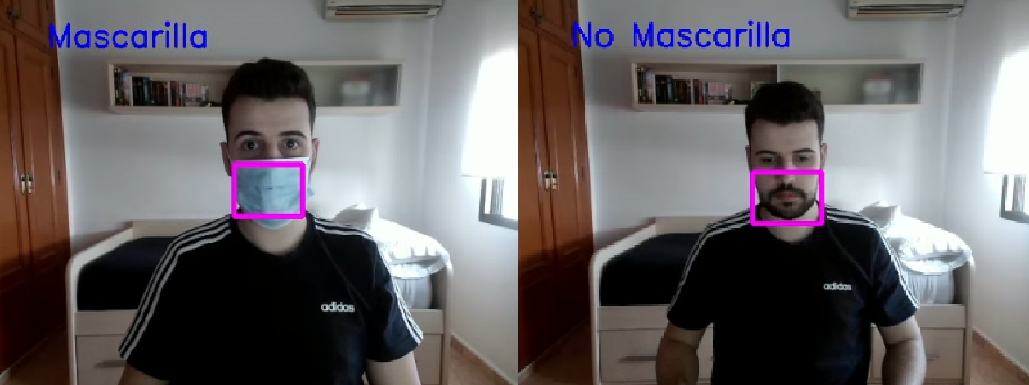
\includegraphics[width=12cm]{imagenes/landmark_prueba.png}
	\caption{Pruebas con Dlib's Facial Landmarks y modelo Haar-like feature \textit{mcs\_mouth.xml}.}
	\label{fig:dlibLandmarks}
\end{figure}

El tiempo de retardo que presenta este prototipo para el PC1 es de una media de 5 ms. Aunque estos tiempos presenten un buen resultado, el funcionamiento del prototipo no es el esperado. Por un lado, le cuesta reconocer un rostro con mascarilla, incluso en muchas ocasiones sin lograrlo, ya en el primer tipo de prueba (distancia de 75 cm). Por otro lado, el detector facial sin mascarilla funciona correctamente y de manera eficaz. Por lo que, otro planteamiento que se podría desarrollar sería un prototipo donde si aparece una detección de una persona y su boca significa que no viste una mascarilla, por tanto no cumpliría con la normativa y saltaría la alarma.

\vspace{-0.8cm}
\subsection*{Próximos pasos}
\vspace{-0.5cm}
En los siguientes apartados se probará implementar prototipos con el uso de Deep Learning. En las últimas décadas, se ha convertido en uno de los métodos mas usados para la creación de aplicaciones de visión artificial. \cite{szeliski_2018}. Esta basado en las estructuras neuronales CNN (\textit{Convolutional Neural Network}), principales responsables de que un ordenador pueda procesar de forma sencilla una imagen. \textit{CNN} es una combinación entre capas neuronales y convolucionales, siendo estas últimas filtros con los que se obtendrán características de la imagen de entrada, los conocidos \textit{features}. La principal función del Deep Learning es clasificar, ya sea una imagen, un objeto o incluso varios objetos a la vez. Esto es gracias al uso de modelos, entrenados con miles de imágenes, que consiguen clasificar imágenes en varias categorías, por ejemplo \textit{MobileNet} \cite{cnn}. 

\newpage
\section{Mediapipe}

Mediapipe es una API \textit{open-source} creada por \textit{Google}, que ofrece servicios de \textit{Machine Learning} para vídeos y fuentes multimedia. Entre ellas, se encuentra un servicio llamado \textit{Face Mesh} que ofrece una solución que estima 468 puntos de interés de un rostro, conformando una malla 3D en tiempo real. Este usa aceleración GPU conjuntamente con un modelo y el uso de una \textit{pipeline}.

La \textit{pipeline} que se utiliza en esta API consiste en dos modelos de \textit{Deep Learning} que trabajan al mismo tiempo. Su funcionalidad es realizar una detección a partir de una imagen de los puntos de interés sobre una cara y construir un modelo \textit{face landmark} 3D que aproxima la superficie de esta mediante regresión sobre dichos puntos. Esta tarea es facilitada si la cara, donde se tienen que detectar los puntos de interés, se encuentra recortada, haciendo así que el modelo se centre solamente en buscar los puntos, aumentando la precisión de la predicción. Asimismo, los recortes de las caras se puede generar a partir de las predicciones anteriores realizadas por el mismo modelo, y solamente es llamada la predicción nuevamente cuando no se consigue detectar la presencia de la cara \cite{faceMesh}.

Todo esto es implementado gracias al framework \textit{MediaPipe}, con la herramienta \textit{MediaPipe graph}. Arquitectura caracterizada por estar formada por componentes llamados \textit{Calculator}, nodos del grafo que tras la entrada de cero o más inputs generan cero o más salidas. Todos estos nodos están conectados mediante datos en forma de \textit{Streams}, donde cada uno representa un conjunto de datos-tiempo en \textit{Packets}. Por tanto, los \textit{calculators} y \textit{steams} definen el flujo de datos del \textit{Graph} \cite{mediapipe}. 

El \textit{pipeline} puede ser definido mediante la adición/modificación de \textit{calculators} dentro del \textit{graph}. Específicamente, el \textit{pipeline} que se utiliza en esta solución (\textit{FaceMesh}) esta formada por un \textit{graph} compuesto por un \textit{subgraph} de \textit{face landmark} (proveniente del módulo, ya implementado, de \textit{face landmark} de \textit{Mediapipe}), donde a su vez usa otro \textit{subgraph} proveniente de \textit{face detection module} para la detección de caras, y un \textit{face renderer subgraph} para mostrar el resultado \cite{faceMesh}. En concreto el \textit{graph} que se usa en esta implementación es el mostrado en la Figura \ref{fig:faceMesh}.

\begin{figure}[htp]
	\centering
	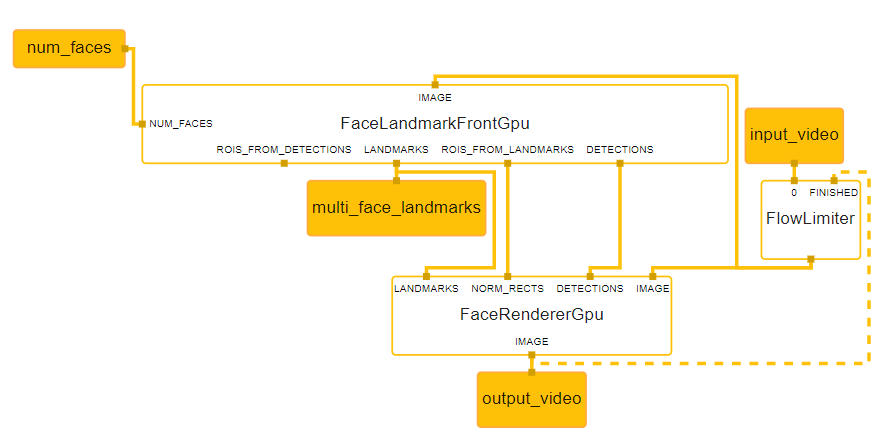
\includegraphics[width=10cm]{imagenes/faceMesh.png}
	\caption{MediaPipe Graph utilizado en FaceMesh \cite{mpGraph}.}
	\label{fig:faceMesh}
\end{figure}

Por tanto, el procesamiento de una imagen en este modelo sigue dos pasos. El primero (1) toma la imagen de entrada, capturada por la cámara, es procesada por un detector de caras \textit{lightweigth}, llamado \textit{BlazeFace}, y produce unos rectángulos que definen el perímetro donde se encuentra la cara, conjuntamente con un par de puntos de interés superficiales (ojos, boca y nariz). Estos puntos se utilizarán para alinear la cara para el siguiente paso. Y el segundo (2), mediante el rectángulo obtenido en el paso anterior, se recorta la cara de la imagen inicial y es re-escalado para utilizarse como entrada de la red neuronal que realiza la predicción de la malla. (El tamaño de re-escalado será entre 256x256 en un modelo completo, hasta 128x128 en el modelo más pequeño). Tras la predicción, se obtiene como salida un vector de coordenadas \textit{landmark 3D}, que serán mapeadas y dibujadas en la imagen original \cite{faceMesh2}. 

Las coordenadas que se obtienen como salida están compuestas por unas coordenadas x e y provenientes de localizaciones del plano 2D propio de la imagen. Mientras que, la coordenada z es interpretada como una profundidad relativa a un centro de masa que compone la malla de la cara.

Se utilizan dos modelos para el funcionamiento de \textit{FaceMesh}. El primero de ellos dedicado a la detección facial, llamado BlazeFace (mencionado anteriormente). Modelo \textit{lightweight} creado para GPU móviles, llegando a una velocidad de procesamiento entre 200 a 1000 fps en dispositivos móviles punteros. Es inspirado en los modelos \textit{MobileNet}, tanto la primera versión como la segunda, provenientes del \textit{framework} SSD (\textit{Single Shot Multibox Detector}). Este modelo produce una salida compuesta por un rectángulo perimetral y 6 puntos de interés faciales. \cite{blazeface}

El segundo modelo, \textit{Face Landmark Model}, generado mediante \textit{Transfer Learning} buscando los siguientes objetivos: crear coordenadas 3D (mencionadas anteriormente) y conseguir mostrarlas en la imagen de salida de forma correcta \cite{faceMesh}. El \textit{Transfer Learning} es una técnica de \textit{Machine Learning} donde se puede hacer uso de un modelo pre-entrenado para personalizarlo y usarlo en una tarea determinada. Conviene destacar que un modelo entrenado es una red almacenada, entrenada previamente con un conjunto de datos con el objetivo de realizar una tarea de clasificación de imágenes a gran escala \cite{transferLearning}.

\textit{FaceMesh} propone una implementación mediante \textit{TensorFlow Lite} que dispone de dos formatos: CPU y GPU, que presentan un rendimiento en dispositivos móviles (\textit{Pixel3}, \textit{Pixel2} y \textit{iPhoneX}) muy fluido, impresionando sobre todo su funcionamiento sobre CPU. (Figura \ref{fig:faceMeshRen}) \cite{faceMesh3}.

\begin{figure}[htp]
	\centering
	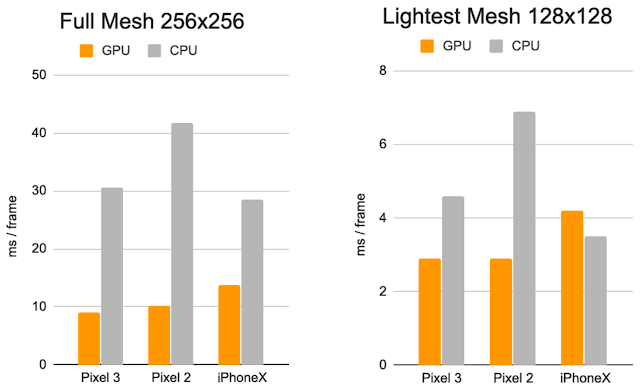
\includegraphics[width=10cm]{imagenes/rendFaceMesh.png}
	\caption{Rendimiento de FaceMesh sobre dispositivos móviles \cite{faceMesh3}.}
	\label{fig:faceMeshRen}
\end{figure}

\vspace{-0.8cm}
\subsection*{Prototipo}
\vspace{-0.5cm}
El prototipo de este apartado se realizará mediante el uso de \textit{FaceMesh} del framework \textit{MediaPipe} y un detector basado en \textit{Haar-like features}, como el mencionado en el \textit{paper} de Viola \& Jones (\ref{haar-like}). Los pasos que lo definen son los siguientes:

\begin{enumerate}
	\item Detección FaceMesh
	
	Para la detección del rostro en la imagen de entrada se utiliza la solución de Mediapipe llamada FaceMesh, implementada en el framework de Python que recibe el mismo nombre, \textit{mediapipe}. Esta solución dispone de dos parámetros de configuración: \textit{min\_detection\_confidence} y \textit{min\_tracking\_confidence}. El primero hace referencia a ..., mientras que el segundo se entiende como ....
	
	Una vez configurado el FaceMesh, se procede a tratar la imagen de entrada para facilitar su tratamiento. Se convierte el espacio de color de la imagen de BGR, espacio de color con el que trabaja \textit{OpenCV}, a RGB. Y, para mejorar el rendimiento, se elimina la opción de la imagen para que sea escribible (\textit{writeable}). Este proceso será invertido después de realizar la detección.
	
	\item Obtención de zona ROI
	
	Tras la detección de Landmarks, el resultado se almacena en una variable llamada \textit{multi\_face\_landmarks}, donde se encuentran todas las marcas faciales de todos los rostros detectados. A su vez, este contiene cada una de las marcas, con una totalidad de 468 puntos.

	Estas marcas contienen parámetros para medir la precisión de la detección del mismo, llamados: \textit{visibility} y \textit{presence}. Si estos valores son muy bajos no se tienen en cuenta. Tras esto, se normalizan sus valores a coordenadas con respecto a los píxeles de la imagen de entrada, se reservan unicamente las coordenadas relacionadas con la boca y se obtiene el ROI donde se localiza esta.
	
	\item Detección de una boca en el ROI 
	
	Para el último paso se hace uso de un modelo pre-entrenado de \textit{Haar-like features} llamado \textit{mcs\_mouth.xml}, capaz de detectar una boca. Si dentro del ROI no se detecta nada, significa que la persona tiene una mascarilla puesta.
\end{enumerate}

Por tanto, la idea tras este prototipo es obtener la zona de la boca gracias al uso de la solución proporcionada por Mediapipe, \textit{FaceMesh}. Y, posteriormente detectar mediante un modelo Haar-like features si existe una boca en dicha zona. Se utiliza la misma idea planteada en el prototipo anterior, pero intentando mejorar su funcionamiento con el uso del framework \textit{Mediapipe}. La desventajas de este prototipo es que si la persona obstaculiza la zona de la boca a la hora de la detección, podría ser capaz de engañar al algoritmo haciendo pensar que si porta una mascarilla, cuando en realidad no es así. Lo bueno es que no hace falta distinguir entre tipos mascarillas.

\begin{figure}[htp]
	\centering
	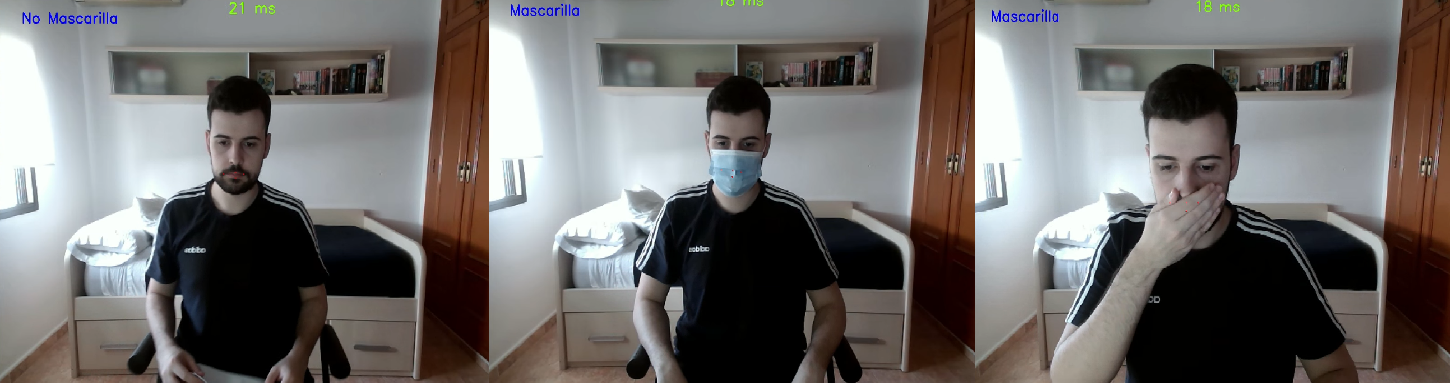
\includegraphics[width=17cm]{imagenes/mediapipe_prueba.png}
	\caption{Pruebas con Mediapipe FaceMesh y modelo Haar-like feature \textit{mcs\_mouth.xml}}
	\label{fig:protoMediapipe}
\end{figure}

El tiempo de retardo que presenta este prototipo para el PC1 es de una media de 15.5 ms. Tras la realización de las pruebas, se puede concluir en que el prototipo funciona de una manera bastante eficaz y precisa en distancias cercanas, mientras que en una posición elevada, como podría ser una puerta, tarda en detectar a la persona, hasta que esta no  se encuentre a una distancia cercana de la misma.

\newpage
\section{Tensorflow}

TensorFlow es una plataforma de \textit{Open Source} dedicada al aprendizaje automático. Permite compilar e implementar con facilidad aplicaciones con tecnología de AA. Esta se basa en tensores, matrices multidimensionales con un tipo uniforme, que si se está familiarizado con NumPy , los tensores son como \textit{np.arrays}. Con la característica de que nunca se puede actualizar el contenido de un tensor, solo crear uno nuevo \cite{tensorflow}.

Concretamente, se usarán los modelos y ejemplos de aprendizaje automático ofrecidos y entrenados mediante la API de alto nivel de Tensorflow para la implementación del último prototipo. Este recurso recibe el nombre de \textit{TensorFlow Model Garden} \cite{modelGarden}, y se trata de un repositorio con diferentes implementaciones de modelos y soluciones modeladas para Tensorflow. Los modelos están pre-entrenados mediante un dataset llamado \textit{COCO 2017} \cite{coco}. Siendo este un gran conjunto de datos a grande escala para \textit{object detection}, segmentación y captación.

Model Garden dispone de un apartado dedicado a la visión artificial, donde se encuentran los ámbitos de clasificación de imágenes, como \textit{MNIST}, \textit{ResNet} o \textit{EfficentNet}, y detección de objetos y segmentación, donde se destacan \textit{RetinaNet}, \textit{Mask R-CNN}, etc. Sin embargo, este prototipo se centrará en la implementación de uno de los modelos que ofrece Model Garden, llamado \textit{SSD-MobileNet}, y aplicar \textit{Transfer Learning} sobre el, para obtener un detector de lo que estamos buscando, comprobar si la mascarilla esta bien vestida.

Transfer Learning es una técnica en la que se reusa un modelo pre-entrenado para un nuevo problema. Últimamente su uso se esta popularizando, ya que permite el entrenamiento de una \textit{deep neural network} con una pequeña cantidad de datos. Algo bastante revolucionario, puesto que todos los modelos hasta ahora necesitaban millones de datos, clasificados a mano y posteriormente necesitar una gran capacidad computacional para ser entrenados \cite{transferLearning}. En este caso, se busca utilizar un modelo general de detección de objetos y aplicando transfer learning, re-entrenarlo para una tarea más especifica pero sin desperdiciar sus conocimientos previos.

\subsection*{SSD-MobileNet}

El prototipo de Tensorflow que se va a construir usará un modelo \textit{SSD-MobileNet}, combinación de un modelo SSD, \textit{Single Shot MultiBox Detector}, con otro llamado MobileNet. Este tipo de modelos se caracterizan por el uso de un método para detectar objetos en imágenes mediante una \textit{deep neural network}, que genera valores de predicción sobre la presencia de cada objeto/categoría en cada una de las detecciones y devuelve el objeto con el que más coincida.

El modelo \textit{SSD} se caracteriza por estar formado por dos componentes principales: un modelo backbone y una cabeza SSD (Figura \ref{fig:ssd}). El backbone es un modelo de clasificación de imágenes, que esta pre-entrenado para ser utilizado como un extractor de características. Normalmente, se implementa con modelos como \textit{ResNet}. Mientras que, la cabeza SSD esta formada por uno o mas capas convolucionales que interpretan la salida del backbone como \textit{bounding boxes} y clases de objetos \cite{ssdwork}. 

\begin{figure}[htp]
	\centering
	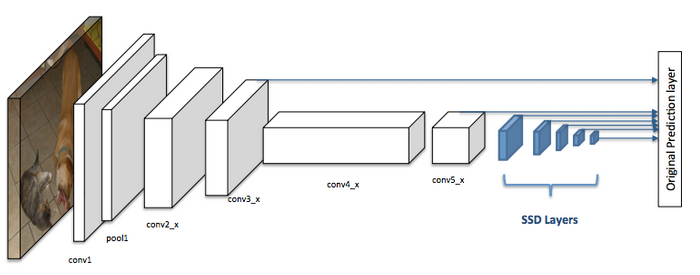
\includegraphics[width=10cm]{imagenes/cnnssd.png}
	\caption{Arquitectura de una CNN con uso de SSD \cite{ssdwork}.}
	\label{fig:ssd}
\end{figure}

Otras característica destacables de SSD es la división de la imagen de entrada mediante un \textit{grid} y realizar una predicción de la clase y la localización del objeto en cada una de las celdas de dicho grid. Si en dicho grid no existe ningún objeto, se considera como \textit{background} y la localización es ignorado. A cada celda se le puede asignar varias \textit{anchor boxes} (\textit{Bounding boxes} con una altura y anchura predefinida) con un tamaño igual al de las celdas. Pero no todos los objetos que están contenidos en la imagen tienen dicho tamaño, por eso se añade un parámetro (\textit{ratio}) dedicado a especificar los diferentes valores que pueden tomar las \textit{anchor boxes}. Asimismo, existe otro parámetro llamado zoom para especificar cuanto pueden escalar dichos \textit{boxes}, tanto aumentando como reduciendo \cite{ssdwork}.

El comportamiento y aportaciones específicas de este modelo, vienen planteadas en el paper con su mismo nombre, \textit{"SSD: Single Shot MultiBox Detector"} \cite{ssd}. Y son las siguientes:

\begin{enumerate}
	\item Se introduce un modelo para la detección de múltiples categorías que es más eficaz y preciso que los modelos posteriores como \textit{YOLO}.
	\item El núcleo de SSD predice la categoría y localización de la \textit{bounding box} mediante el uso de pequeños filtros convolucionales aplicados sobre mapas de características.
	\item Para obtener una mayor precisión se realizan predicciones sobre mapas de características con diferente escalado.
	\item Experimentación con análisis de tiempo y precisión sobre el modelo evaluado sobre \textit{PASCAL VOC}, \textit{COCO} y \textit{ILSVRC}. Asimismo, es comparado con modelos recientes.
\end{enumerate}

MobileNet es un modelo con arquitectura \textit{CNN} para la clasificación de imágenes y visión artificial en móviles. Lo que hace especial este modelo es la potencia computacional necesaria para ejecutarlo o aplicar transfer learning sobre el. Esto lo convierte en un perfecto candidato para dispositivos móviles, sistemas integrados y ordenadores sin GPU o baja eficiencia computacional sin llegar a comprometer significativamente la precisión de los resultados.

Este modelo se basa en el uso de una arquitectura optimizada que utiliza convoluciones separables en profundidad para construir \textit{deep neural networks} ligeros. Además, proporciona dos hiperparámetros globales que permiten ajustar de forma eficiente entre la latencia y precisión. Por consiguiente, con la combinación de ambos, se logra la creación de un modelo apto para dispositivos y ordenadores con poca potencia de GPU, capaz de obtener una detección de forma precisa y veloz.

\newpage
\subsection*{Prototipo}

\begin{enumerate}
	\item Instalación del framework
	
	Para realizar este prototipo se hace uso del API \textit{object\_detection} proporcionado por Tensorflow para Python. Tras seguir las instrucciones ofrecidas se consigue un entorno de trabajo con las siguientes herramientas: Anaconda conjunto a una versión de Python 3.7, Tensorflow, CUDA, TensorFlow Model Garden,  Object Detection API, Protobuf y COCO API.
	
	\item Elección del modelo
	
	A la hora de elegir un modelo se tienen en cuenta dos parámetros principales: 
	
	\begin{itemize}
		\item Coco mAP (\textit{main Average Prestion}): indica la precisión media del modelo.
		\item Speed: velocidad de refresco.
	\end{itemize} 
	
	\textit{\textbf{SSD-MobileNetV2}} (320x320) será el modelo elegido, ya que dispone de las mejores medidas en cuanto a velocidad. Exactamente cuenta con una medida \textit{Coco mAP} de 20.2 y 19 ms de \textit{Speed}. Aunque la precisión sea más baja que el resto de modelos, se suple con la gran velocidad que logra este modelo.
	
	\item Dataset de imágenes y labeling
	
	%https://arxiv.org/abs/2008.08016
	%https://www.kaggle.com/prithwirajmitra/covid-face-mask-detection-dataset#
	
	Para el dataset, he realizado una serie de fotos con varias mascarillas y sin (todas estas imágenes son tomadas con la webcam que se va a realizar el trabajo) mezcladas con imágenes de ejemplo encontradas por internet. Consta de un total de X imágenes, dividas en dos grupos train y test. En el primero se encuentran las imágenes que se utilizarán para el entrenamiento del modelo por \textit{Transfer Learning} y cuenta con X imágenes. Mientras que, el conjunto de test se utilizará para validar el modelo entrenado con un total de X imágenes.
	
	Para construir un dataset más completo se utiliza una técnica llamada \textit{Data Argumentation}, que genera modificaciones de las imágenes del modelo, como blur, rotaciones, etc.
	
	Antes de realizar el modelo es necesario preparar las imágenes conjuntamente a un archivo donde se plasmen las etiquetas del modelo. Para ello, se hace uso de un programa (hecho en Python) llamado \textit{labelImg}. Al tratar las imágenes, se crean unos archivos \textit{xml} donde se encuentra la información del etiquetado que se ha realizado, en este caso se tiene uno de los dos labels del trabajo: \textit{mask} o \textit{noMask}. Una vez creados todos los archivos de etiquetado \textit{xml} con los labels, se tiene que crear un archivo \textit{pbtxt} donde se refleje todas las labels posibles que tendrá el modelo.
	
	En resumen, un \textit{LabelMap} es una archivo referido a enumerar todas las clases posibles en la identificación de objetos. Además, cada una de las imágenes de entrenamiento dispondrá de un archivo adicional donde aparezcan cada \textit{label} de la misma y su localización. Depende del modelo usado, los archivos de \textit{LabelMap} serán de un tipo u otro. En el caso de Tensorflow se utiliza un \textit{TFRecord}, mientras que en YOLO se usa un \textit{txt}.
	
	 Por último, se usa un script proporcionado por Tensorflow para transformar el etiquetado que hemos realizado al formato correcto para el entrenamiento del modelo (\textit{TFRecord}).
	
	\item Transfer Learning
	
	Antes de hacer el entrenamiento se tiene que preparar un archivo de configuración sobre el modelo seleccionado (SSD-MobileNetV2). Este archivo tiene el nombre de \textit{pipeline.config} y contiene la información principal del modelo, tanto el número de clases que puede detectar, el tamaño que reajusta las imágenes antes de tratarlas y checkpoints para el entrenamiento. Para su creación será necesario el uso de las siguientes herramientas: Tensorflow, Object Detection API y Protobuf. Este último, es una herramienta de Google centrada en transformar los \textit{xml} de etiquetado que hemos creado antes en \textit{protocol buffers}, para poder serializar la información de forma estructurada y más rápida.
	
	Para realizar el entrenamiento se hace uso del código proporcionado tras la instalación de la API Object Detection de Tensorflow, llamado \textit{model\_main\_tf2}. A este hay que cederle la siguiente información: dirección de salida, archivo de configuración y número de pasos de entrenamiento. Tras el entrenamiento, se obtienen unos archivos llamados \textit{checkpoints} con los que se podrá cargar el modelo para su uso mediante la siguientes clases de Tensorflow: \textit{Model\_builder} y \textit{Checkpoint}.
	
	\item Realizar detección
	
	Para la detección de la mascarilla se crea una función, \textit{detect\_fn}, que tomando una imagen se pre-procesa con el objetivo de  reducir su tamaño al de la entrada del modelo, siendo en este caso 320x320. Tras esto, se realiza la detección usando el modelo que hemos creado y se realiza un post-procesado para obtener una imagen de salida del mismo tamaño que la de entrada.
	
	El último paso será realizar esta detección en tiempo real, mediante el uso de OpenCV. Una vez capturado un \textit{frame} de la cámara de entrada, se debe transformar en una entrada compatible con el modelo, en este caso un tensor. Con este ya se puede detectar el objeto con la función que se ha definido anteriormente, \textit{detect\_fn}. 
	
	De manera que, cuando se obtiene el label que se ha detectado, se utiliza la herramienta de visualización de la API Object Detection, \textit{visualization\_utils}, para mostrar el resultado por pantalla. Un ejemplo del funcionamiento se puede observar en la \textit{Figura \ref{fig:protoTensorFlow}}.
\end{enumerate}

\begin{figure}[htp]
	\centering
	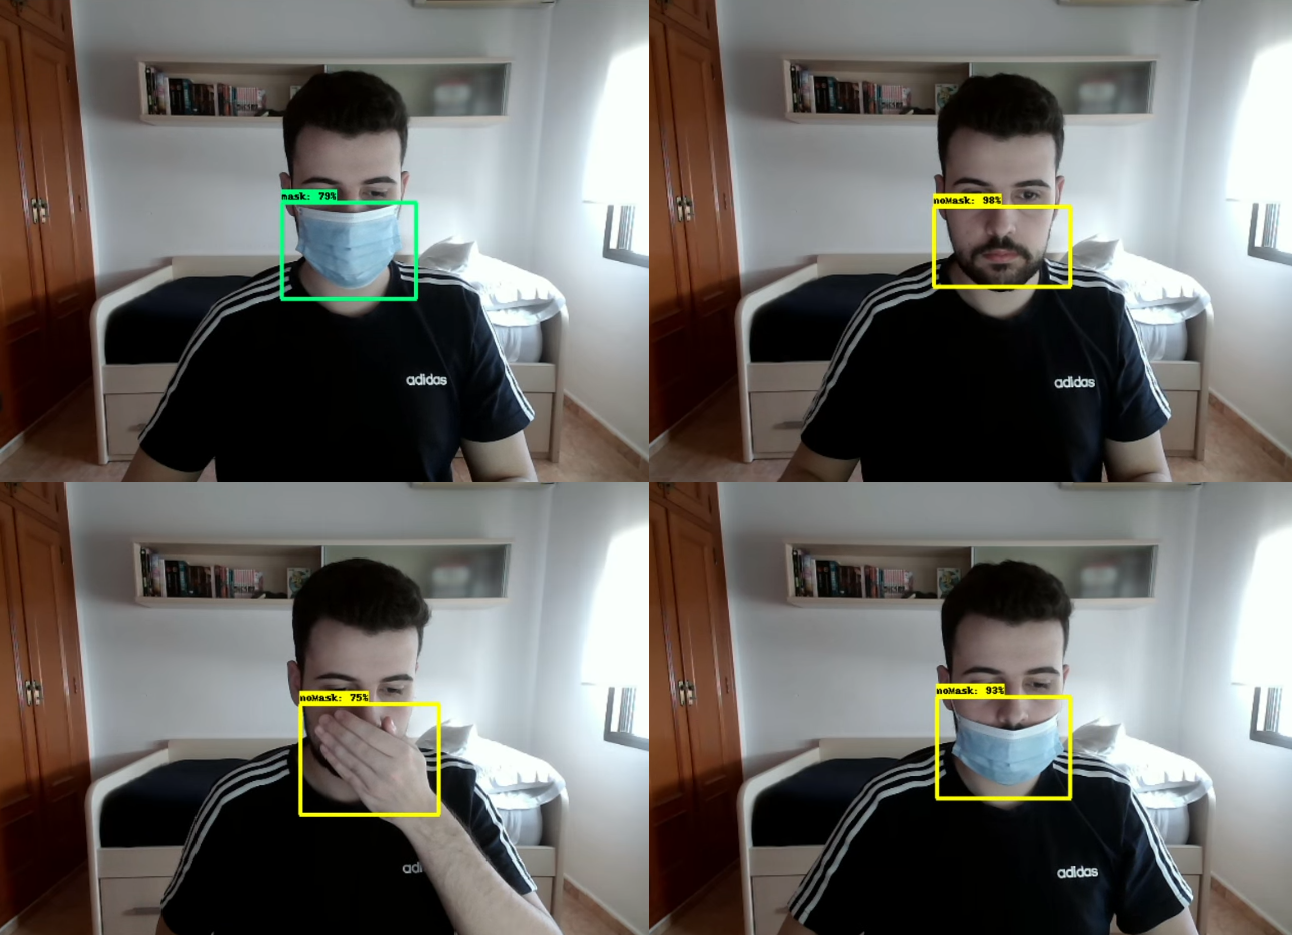
\includegraphics[width=12cm]{imagenes/tf_prueba.png}
	\caption{Pruebas con SSD-MobileNetV2 \textit{mcs\_mouth.xml}}
	\label{fig:protoTensorFlow}
\end{figure}

\newpage
El tiempo de retardo que presenta este prototipo para el PC1 es de una media de 83.2 ms. Aunque el resultado obtenido sea bastante bueno, solamente funciona en un ámbito cerrado. Esto se debe a que el entrenamiento del modelo usado se ha realizado con imágenes mías. Aun así, este prototipo, al igual que los anteriores, funciona de forma correcta y precisa en pruebas cercanas a la cámara, mientras que en distancias mayores se dificulta la detección. De igual forma, si se encuentra en una situación donde la iluminación sea escasa o la cámara no este bien colocada el rendimiento del prototipo disminuye.

%\subsection{Prototipo RetinaNet}

%Explicar RetinaNet y pruebas

%\subsection{Prototipo YOLO}

%Explicar YOLO y pruebas
%https://medium.com/analytics-vidhya/yolov3-custom-object-detection-with-transfer-learning-47186c8f166d
%https://github.com/hunglc007/tensorflow-yolov4-tflite


\newpage
\section{Comparación}